\documentclass[margin=0px]{article}

\usepackage{listings}
\usepackage[utf8]{inputenc}
\usepackage{graphicx}
\usepackage{float}
\usepackage[a4paper, margin=1in]{geometry}
\usepackage{subcaption}
\usepackage{amsthm}
\usepackage{amssymb}
\usepackage{amsmath}

\renewcommand{\figurename}{ábra}
\newenvironment{tetel}[1]{\paragraph{#1 \\}}{}

\newcommand{\N}{\mathbb{N}}
\newcommand{\Z}{\mathbb{Z}}
\newcommand{\R}{\mathbb{R}}
\newcommand{\Q}{\mathbb{Q}}
\newcommand{\C}{\mathbb{C}}

% A dokument itt kezdődik

\title{Záróvizsga tételsor \\ \large 4. Számelmélet, gráfok, kódoláselmélet}
\date{}
\author{Dobreff András}

\begin{document}
	\maketitle
	
	\begin{tetel}{Számelmélet, gráfok, kódoláselmélet}
			Relációk, rendezések. Függvények és műveletek. Számfogalom, komplex számok. Leszámlálások véges halmazokon. Számelméleti alapfogalmak, lineáris kongruencia-egyenletek. Általános és síkgráfok, fák, Euler- és Hamilton-gráfok, gráfok adatszerkezetei. Polinomok és műveleteik, maradékos osztás, Horner-séma. Betűnkénti kódolás, Shannon- és Huffman-kód. Hibajavító kódok, kódtávolság. Lineáris kódok.
	\end{tetel}
	\section{Számelmélet}
		\subsection{Relációk, rendezések}
			\begin{description}
				\item[Alapfogalmak] \hfill
					\begin{itemize}
						\item Rendezett pár \\
							$(x,y)$ rendezett pár, ha $(x,y) = (u,v) \Longleftrightarrow x = u \ \land \ y = v$. Ezt a tulajdonságot halmazokkal definiáljuk:
							\[ (x,y) := \{ \{x\}, \{x, y\} \} \]
						\item Descartes-szorzat \\
							$X,Y$ halmazok Descartes-szorzata vagy direkt szorzata:
							\[ X \times Y := \{ (x,y) : x \in X, y \in Y \} \]
						\item Binér reláció \\
							Egy halmazt binér relációnak nevezünk, ha minden eleme rendezett pár. 
							Ha $R$ binér reláció és $(x,y) \in R$, akkor gyakran írjuk: $xRy$
						\item Reláció \\
							Ha $X,Y$ halmazokra $R \subset X\times Y$, akkor $R$ reláció $X$ és $Y$ között.
						\item Értelmezési tartomány \\
							Az $R$ binér reláció értelmezési tartománya:
							\[ \textrm{dmn}(R) := \{ x\  | \ \exists y : (x,y)\in R  \}\]
						\item Érték készlet \\
							Az $R$ binér reláció érték készlete:
							\[ \textrm{rng}(R) := \{ y\  | \ \exists x : (x,y)\in R  \}\]
						\item Inverz \\
							Egy $R$ binér reláció inverze:
							\[R^{-1} := \{(a,b) : (b,a) \in R\} \]
						\item Halmaz képe \\
							Legyen $R$ binér reláció, és $A$ halmaz. Az $A$ halmaz képe:
							\[R(A) := \{y \ | \ \exists x\in A: (x,y) \in R\} \]
						\item Kompozíció \\
							$R$ és $S$ binér relációk kompozíciója:
							\[ R \circ S := \{ (x,y) \ | \ \exists z : (x,z) \in S \ \land \ (z,y) \in R \ \} \]
					\end{itemize}
				\item[Tulajdonságok] \hfill \\
					Az $R$ egy $X$-beli binér reláció (azaz $R \subset X\times X$)
					\begin{enumerate}
						\item tranzitív \\
							\[\forall x,y,z : (x,y)\in R \ \land \ (y,z) \in R \Longrightarrow (x,z) \in R \]
						\item szimmetrikus \\
							\[\forall x,y : (x,y)\in R \Longrightarrow (y,x) \in R \]
						\item antiszimmetrikus \\
							\[\forall x,y : (x,y)\in R \ \land \ (y,x) \in R \Longrightarrow x = y\]
						\item szigorúan antiszimmetrikus \\
							\[\forall x,y : (x,y)\in R \Longrightarrow (y,x) \notin R\]
						\item reflexív \\
							\[\forall x \in X : (x,x)\in R\]
						\item irreflexív \\
							\[\forall x \in X : (x,x)\notin R\]
						\item trichotóm \\
							Ha minden $x,y \in X$ esetén az alábbiak közül pontosan egy teljesül
							\begin{enumerate}
								\item[a)] $x=y$
								\item[b)] $(x,y) \in R$
								\item[c)] $(y,x) \in R$
							\end{enumerate}
						\item dichotóm \\
							\[\forall x,y \in X : (x,y) \in R \ \lor \ (y,x) \in R\]
							Más néven az elemek összehasonlíthatóak.
					\end{enumerate}
				\item[Rendezések] \hfill
					\begin{itemize}
						\item Ekvivalenciareláció, osztályozás \\
							$X$ halmaz, $R$ $X$-beli binér reláció ekvivalenciareláció, ha
							\begin{itemize}
								\item Reflexív
								\item Tranzitív
								\item Szimmetrikus
							\end{itemize}
							
							$X$ részhalmazainak egy $\mathcal{O}$ rendszerét osztályozásnak hívjuk, ha $\mathcal{O}$ páronként diszjunkt nemüres halmazokból álló halmazrendszer, melyre $\cup\mathcal{O} = X$ 
							\\\\
							Tétel: \\
							Egy ekvivalenciareláció meghatároz egy osztályozást. Fordítva: $\mathcal{O}$ osztályozásra \\ ${R = \cup\{Y\times Y : Y \in \mathcal{O} \}}$ ekvivalenciareláció.
							
						\item Részbenrendezés\\
							$X$ halmaz, $R$ $X$-beli binér reláció részbenrendezés, ha
							\begin{itemize}
								\item Reflexív
								\item Tranzitív
								\item Antiszimmetrikus
							\end{itemize}
						\item Teljes rendezés \\
							$X$ halmaz, $R$ $X$-beli binér reláció (teljes) rendezés, ha
							\begin{itemize}
								\item Reflexív
								\item Tranzitív
								\item Antiszimmetrikus
								\item Dichotóm
							\end{itemize}
							Magyarul ha egy részbenrendezés dichotóm (tehát minden eleme összehasonlítható), akkor (teljes) rendezés.
						\item Szigorú és gyenge reláció, rendezés \\
							$X$ halmaz, $R$,$S$ relációk $X$-beliek. Ha
							\[ xRy \ \land \ x \neq y \Rightarrow xSy\]
							akkor $S$-et az $R$ szigorításának nevezzük.\\
							Megfordítva, ha
							\[  xRy \ \lor \ x = y \Rightarrow xTy \]
							akkor $T$ az $R$-hez megfelelő gyenge reláció.\\
							
							\textit{Megjegyzés: Tulajdonképpen a reflexívitás elvételéről és hozzáadásáról van szó. Egy részbenrendezés esetén a megfelelő szigorú reláció (szigorú részbenrendezés) tehát irreflexív, következésképpen szigorúan antiszimmetrikus is. Megfordítva: Egy X-beli szigorú részbenrendezés (tran., irrefl., szig. ant.) megfelelő gyenge relációja részbenrendezés. }
					\end{itemize}
				\item[Korlátok] \hfill 
					\begin{itemize}
						\item Legkisebb, legnagyobb, minimális, maximális elem \\
							$X$ halmazbeli részbenrendezés ($\preccurlyeq$) legkisebb (legelső) elemén egy olyan $x\in X$ elemet értünk, melyre: $\forall y \in X : x\preccurlyeq y$. (Ilyen nem biztos, hogy létezik, de ha igen, akkor egyértelmű).\\
							Hasonlóan a legnagyobb (utolsó) elem olyan $x\in X$, hogy $\forall y \in X : y \preccurlyeq x$.\\
							
							$x$-et minimálisnak nevezzük, ha nincs nála kisebb elem, maximálisnak, ha nincs nála nagyobb elem. (Szemben a legkisebb/legnagyobb elemekkel, minimális/maximális elemből több is lehet. Ha viszont $X$ rendezett, akkor legkisebb=minimális, legnagyobb=maximális.)
						\item Alsó, felső korlát \\
							$X$ részbenrendezett halmaz, $Y \subset X$. Az $x \in X$ elem az $Y$ alsó korlátja $\forall y \in Y : x \preccurlyeq y$. (felső korlátja: $\forall y \in Y : y \preccurlyeq x$). Látható, hogy $x$ nem feltétlenül eleme $Y$-nak, sőt az is lehet, hogy $Y$-nak nincs alsó/felső korlátja, vagy akár több is van. Ha azonban $x\in Y$, akkor egyértelmű és ez Y legkisebb eleme.
						\item Infimum, szuprémum \\
							Ha az alsó korlátok között van legnagyobb elem, azt $Y$ alsó határának, infimumának nevezzük. (Jele: inf$Y$) \\
							Ha a felső korlátok között van legnagyobb elem, azt $Y$ felső határának, szuprémumának nevezzük. (Jele: sup$Y$)
						\item Alsó, felső határ tulajdonság \\
							$X$ részbenrendezett halmaz. Ha $ \forall \emptyset \neq Y \subset X$ : $Y$ felülről korlátos és van szuprémuma, akkor felső határ tulajdonságú.
							Illetve ha $ \forall \emptyset \neq Y \subset X$ : $Y$ alulról korlátos és van infimuma, akkor alsó határ tulajdonságú.
					\end{itemize}
			\end{description}
		\subsection{Függvények és műveletek}
			\subsubsection{Függvények}
				\begin{description}
					\item[Definíció] \hfill \\
						Egy $f$ reláció függvény, ha
						\[ (x,y) \in f \ \land (x,y') \ \in f \Longrightarrow y = y' \]
						Más szóval minden $x$-hez legfeljebb egy olyan $y$ létezik, hogy $(x,y) \in f$
						
						Így minden $x \in$ dmn($f$)-re az $f(x) = \{y\}$, melyet $f(x) = y$ vagy $f: x \mapsto y$ vagy $f_x = y$ is szoktunk jelölni.
						
					\item[Értelmezési tartomány, értékkészlet] \hfill \\
						Az $f : X \rightarrow Y$ jelölést használjuk, ha dmn($f$) $ = X $. \\
						Az $f \in X \rightarrow Y$ jelölést használjuk, ha dmn($f$) $\subset X$ (amikor dmn($f$)$ \subsetneq X$ is előfordulhat).\\
						Mindkét esetben rng($f$) $\subset Y$.
							
					\item[Injektív] \hfill \\
						$f$ függvény kölcsönösen egyértelmű/injektív, ha 
						\[ f(x) = y \ \land \ f(x') = y \ \Longrightarrow \ x = x' \]
						Ez azzal ekvivalens, hogy $f^{-1}$ reláció is függvény.
					\item[Szürjektív] \hfill \\
						Az $f$ függvény szürjektív, ha
							\[ \forall y \in Y : \exists x\in X : f(x) = y\]
							Azaz rng($f$) = $Y$. Magyarul az $f$ függvény az egész $Y$-ra képez.
					\item[Bijektív] \hfill \\
						Ha az $f$ függvény injektív és szürjektív, akkor bijektív.
					\item[Indexelt család] \hfill \\
						Az $x$ függvény $i$ helyen felvett értékét $x_i$-vel is szoktuk jelölni. Ilyenkor gyakran dmn($f$) = $I$ értelmezési tartományt indexhalmaznak, elemeit indexeknek, rng($f$)-et indexelt halmaznak, és magát az $x$ függvényt indexelt családnak szoktuk nevezni.
				\end{description}
			\subsubsection{Műveletek}
				\begin{description}
					\item[Definíciók] \hfill
						\begin{itemize}
							\item Binér művelet \\
								$X$ halmazon egy $f : X \times X \rightarrow X$ függvény binér művelet.
							\item Unér művelet \\
								$X$ halmazon egy $f : X \rightarrow X$ függvény unér művelet.
							\item Nullér művelet \\
								$X$ halmaz, $f : \{\emptyset \} \rightarrow X $ nullér művelet. (Gyakorlatilag elemkiválasztás)
						\end{itemize}
					\item[Tulajdonságok] \hfill
						\begin{itemize}
							\item Legyen $\spadesuit, \copyright$ binér műveletek $X$-en. 
								\begin{enumerate}
									\item $\spadesuit$ asszociatív, ha
									\[ \forall x,y,z \in X : \quad (x \ \spadesuit \ y ) \ \spadesuit \ z = x \  \spadesuit \  (y \ \spadesuit z) \]
									
									\item $\spadesuit$ kommutatív, ha
									\[ \forall x,y \in X : \quad x \ \spadesuit \ y = y \  \spadesuit \  x \]
									
									\item $\spadesuit$ disztributív a $\copyright$-ra, ha $\forall x,y,z \in X$:
									\[ x \  \spadesuit \  (y \ \copyright \ z) = (x \  \spadesuit \ y) \ \copyright \ (x \ \spadesuit \ z) \quad \textrm{ - baloldali} \]
									\[ (y \ \copyright \ z) \  \spadesuit \ x = (y \  \spadesuit \ x) \ \copyright \ (z \ \spadesuit \ x) \quad \textrm{ - jobboldali} \]
								\end{enumerate}
								
							\item Legyen $\heartsuit$ binér művelet $X$-en és $\S$ binér művelet $Y$-on
							$f : X \rightarrow Y$ művelettartó ha:
							\[ \forall x_1,x_2 \in X:  f(x_1 \heartsuit x_2) = f(x_1) \ \S \ f(x_2) \]
						\end{itemize}
				\end{description}
		\subsection{Számfogalom, komplex számok}
			\subsubsection{Számfogalom}
				\begin{description}
					\item[Algebrai Struktúrák] \hfill
						\begin{enumerate}
							\item Grupoid \\
								$G$ halmaz egy $\star$ művelettel, azaz a $(G, \star)$ párt grupoidnak nevezzük.
							\item Félcsoport\\
								Ha egy grupoidban a $\star$ művelet asszociatív, akkor a grupoid félcsoport.
							\item Monoid \\
								Semleges elemes félcsoportot monoidnak nevezzük.\\
								\textit{Megyjegyzés: $ a \in G$ semeleges elem, ha $\forall g \in G : a \star g = g \star a = g$}
							\item Csoport \\
								Ha egy monoidban minden elemnek van inverze, akkor csoportról beszélünk. \\
								\textit{Megyjegyzés: $g,g^{-1} \in G$ és $\xi\in G$ semleges elem, akkor a $g^{-1}$ a $g$ inverze, ha $g\star g^{-1} = \xi$ és $g^{-1} \star g = \xi$}
							\item Ábel-csoport \\
								Ha egy csoportban a művelet kommutatív, akkor Abel-csoport.
							\item Gyűrű \\
								$(R,+,\cdot )$ gyűrű, ha az összeadással Abel-csoport, a szorzással félcsoport és teljesül mindkét oldali disztributivitás.
								
								Ha a szorzás kommutatív, akkor kommutatív gyűrű. 
								
								Ha a szorzásnak van egységeleme, akkor egységelemes gyűrű.
							\item Integritási tartomány \\
								Nullosztó mentes kommutatív gyűrű.
								
								\textit{Nullosztó: $x,y$ nullátók különböző elemek, de $x\cdot y = 0$}
							\item Rendezett integritási tartomány \\
								$R$ integritási tartomány rendezett integritási tartomány, ha rendezett halmaz, továbbá az összeadás és szorzás monoton.
								
								\textit{Összeadás monoton: $x,y,z \in R$ és $x \leq y \ \Rightarrow \ x+z \leq y+z$ \\ 
									Szorzás monoton: $x,y \in R$ és $x,y\geq0 \ \Rightarrow \ x\cdot y \geq 0$ }
							\item Test \\
								Egy $R$ gyűrűt, ha $R\setminus\{0\}$ szorzással Abel-csoport, akkor test.
							\item Rendezett test \\
								Ha egy test rendezett integritási tartomány, akkor rendezett test.
						\end{enumerate}
					\item[Természetes számok]\hfill
						\begin{itemize}
							\item Peano-axiómák \\
								Legyen $\N$ egy halmaz és a $^+$ egy $\N$-en értelmezett függvény. Az alábbi feltételeket Peano-axiómáknak nevezzük:
								\begin{enumerate}
									\item $0 \in \N \qquad$ - $0$ egy nullér művelet $\N$-en
									\item ha $n \in \N$, akkor $n^+ \in N \qquad$ - $^+$ egy unér művelet $\N$-en
									\item ha $n \in \N$, akkor $n^+ \neq 0 \qquad $ - $0$ nincs a $^+$ értékkészletében
									\item ha $n,m \in \N$, és $m^+ = n^+$, akkor $n = m \qquad $ - $^+$ injektív
									\item ha $S \subset \N, 0 \in S$, továbbá $ n \in S : n^+\in S$, akkor $S = \N \qquad $ - a matematikai indukció elve  
								\end{enumerate}
							\item Műveletek
								\begin{itemize}
									\item összeadás \\
										$k,m,n \in \N$, akkor:
										\begin{enumerate}
											\item $(k+m)+n = k+(m+n)$ \textit{- asszociativitás}
											\item $n+0 = 0+n = n$ \textit{- 0 a nullelem (additív semleges elem)}
											\item $n+k = k+n$ \textit{- kommutativitás}
											\item $n+k = m+k$ vagy $k+n = k+m$, akkor $m=n$ \textit{- egyszerűsítési szabály}
										\end{enumerate}
									\item szorzás \\
										$k,m,n \in \N$, akkor:
										\begin{enumerate}
											\item $(k\cdot m)\cdot n = k\cdot (m\cdot n)$ \textit{- asszociativitás}
											\item $ 0\cdot n = n\cdot 0 = 0$
											\item $n\cdot 1 = 1\cdot n = n$ \textit{- 1 az egységelem (multiplikatív semleges elem)}
											\item $n\cdot k = k\cdot n$ \textit{- kommutativitás}
											\item $k\cdot (m+n) = k\cdot m + \cdot n$, illetve $(m+n) \cdot k = m\cdot k+n\cdot k$ \textit{- disztributivitás}
											\item $k\neq 0$ esetén: $n\cdot k = m\cdot k$, akkor $m=n$ \textit{- egyszerűsítési szabály}
										\end{enumerate}
								\end{itemize}
						\end{itemize}
					\item[Egész számok] \hfill \\
						Természetes számok körében az összeadásra nézve csak a nullának van inverze, másként szólva, a kivonás általában nem végezhető el. 
						
						Tekintsük a $\sim\ \subset\N\times\N$ relációt, melyre $(m,n) \sim (m',n')$, ha $m+n' = m'+n$. És vegyük az $(m,n)+(m',n') = (m+m',n+n')$ összeadást. A $\sim$ reláció ekvivalenciareláció, az ekvivalenciaosztályok halmazát jelöljük $\Z$-vel. $\Z$ elemeit egész számoknak nevezzük.
						
						Az összeadás kompatibilis az ekvivalenciával, így az egész számok között értelmezve van, és $(\Z, +)$ Ábel-csoport.
						
						Tehát $(\Z, +, \cdot)$ gyűrű.
						
						\textit{Megjegyzés: $*$ művelet kompatibilis a $\asymp$ ekvivalenciarelációval, ha teljesül: $ x \asymp x' \ \land \ y \asymp y' \ \Longrightarrow \ x * y \asymp x'*y'$}
					\item[Racionális számok] \hfill \\
						Az egész számok körében a nem nulla elemek közül csak az 1-nek és a $-1$-nek van multiplikatív inverze, másként szólva az osztás általában nem végezhető el.
						
						Tekintsük a $\Z \times (\Z\setminus\{0\})$-n a $\sim$ relációt, melyre $(m,n) \sim (m',n')$, ha $mn' = nm'$. És vegyük az $(m,n)+(m',n') = (mn'+nm', nn')$ összeadást és az $(m,n)\cdot(m',n')=(mm', nn')$ szorzást. A $\sim$ reláció ekvivalenciareláció, az ekvivalenciaosztályok halmazát jelöljük $\Q$-val. $\Q$ elemeit racionális számoknak nevezzük.  
						
						$(\Q, +, \cdot)$ rendezett test.
					\item[Valós számok] \hfill \\
						Nincs olyan $a \in \Q$ szám, melynek négyzete 2. Tehát nem minden szám írható fel m/n ($m,n \in \N^+$) alakban.
						
						Archimédeszi rendezettség:\\
						Egy $F$ rendezett testet archimédeszien rendezett, ha $x,y\in F: \exists n \in \N : nx \geq y \quad (x>0)$
						
						A racionális számok rendezett teste archimédeszien rendezett, de nem felső határ tulajdonságú.
						
						Egy felső határ tulajdonságú rendezett testet a valós számok testének nevezünk, és $\R$-rel jelöljük. ($\exists!\R$)
				\end{description}
			\subsubsection{Komplex számok}
				A komplex számok szükségét a harmadfokú egyenletek megoldására való Cardano-képlet szülte. Ugyanis abban az esetben, amikor az egyenletnek három különböző valós gyöke van, a képletben a gyökjel alá negatív szám kerül. Fokozatosan tisztult a "képzetes" számokkal való számolás szabályai, és a trigonometrikus függvényekkel való kapcsolat.
				
				\begin{description}
					\item[Definíció] \hfill \\
						A komplex számok halmaza $\C = \R \times \R$. $\C$ az $(x,y)+(x',y') = (x+x', y+y')$ összeadással és az $(x,y)\cdot(x',y') = (xx'-yy', y'x+yx')$ szorzással test. A komplex számok halmaza nem rendezett test, mivel (tétel alapján) egy rendezett integritási tartományban $ x \neq 0 \ \Rightarrow x^2 > 0$. (Ez azonban $(0,1)^2=i^2 = -1$-re nem teljesül). 
						
						[A komplex számok körében (0,0) a nullelem, $(1,0)$ egységelem, $(x,y)$ additív inverze $(-x,-y)$, és $(0,0) \neq (x,y)$ pár multiplikatív inverze az $(\frac{x}{x^2+y^2}, \frac{-y}{x^2+y^2})$ pár.]
					\item[Valós számok azonosítása] \hfill \\
						Mivel $(x,0)+(x',0) = (x+x',0)$ és $(x,0)\cdot(x',0) = (xx',0)$ így az összes $(x,0), x\in\R$ komplex számot azonosíthatjuk $\R$-rel.
					\item[Komplex számok algebrai alakja] \hfill \\
						Mivel
						\[(x,y) = (x,0)+(y,0)\cdot i = x+yi\]
						így a komplex számokat $a+bi$ algebrai alakban is írhatjuk.
						
						Ekkor az Re($z$) = $x$ valós számot a $z = (x,y)$ komplex szám valós részének, az Im($z$) = $y$ valós számot pedig a képzetes  részének nevezzük.
					\item[Konjugált] \hfill \\
						$ z = x+yi$ komplex szám konjugáltja: $\overline{z} = x-yi$
						
						Tulajdonságai:
						\begin{enumerate}
							\item $\overline{z+w} = \overline{z}+\overline{w}$
							\item $\overline{z\cdot w} = \overline{z}\cdot\overline{w}$
							\item $\overline{\overline{z}} = z$
							\item $z + \overline{z}$ = 2Re($z$)
							\item $z - \overline{z}$ = $i\cdot2$Im($z$)
						\end{enumerate}
					\item[Abszolút érték] \hfill \\
						A $z=(x,y)$ komplex szám abszolút értéke: $|z| = \sqrt{x^2+y^2}$
					
						Tulajdonságai:
						\begin{enumerate}
							\item $z\cdot\overline{z} = {|z|}^2$
							\item $\frac{1}{z}= \frac{\overline{z}}{|z|^2} $
							\item $|z| = \overline{|z|}$
							\item $|z\cdot w | = |z|\cdot|w|$
							\item $|z+w| \leq |z| +|w|$
						\end{enumerate}
					\item[Trigonometrikus alak] \hfill
						\begin{itemize}
							\item Argumentum \\
								$z \neq 0$ esetén az a $z$ argumentuma $\forall t \in\R$, melyre Re($z$) = $|z|$cos($t$), és Im($z$) = $|z|$sin($t$). Más szóval a $z$ argumentuma az origóból a $z$-be mutató vektor és a pozitív valós tengellyel bezárt szöge.
							\item Trigonometrikus alak \\
								A $z$ komplex szám trigonometrikus alakja: $ z = |z|($cos($t$)+$i\cdot$sin($t$)
							\item Moivre-azonosságok \\
								Legyen $z = |z|($cos($t$)+$i\cdot$sin($t$)), és $w = |w|($cos($s$)+$i\cdot$sin($s$)). Ekkor
								\[z\cdot w = |z||w|(\textrm{cos}(t+s)+i\cdot \textrm{sin}(t+s))\]
								\[\frac{z}{w} = \frac{|z|}{|w|}(\textrm{cos}(t-s)+i\cdot \textrm{sin}(t-s)) \quad (w \neq 0)\]
								\[ z^n = |z|^n(\textrm{cos}(nt)+i\cdot \textrm{sin}(nt)) \quad (n \in \Z)\]
							\item Gyökvonás \\
								Legyen $z^n = w$ ekkor:
								\[ \sqrt[n]{w} = \Bigg\{z_k = \sqrt[n]{|w|}\bigg(\textrm{cos}\Big(\frac{t+2k\pi}{n}\Big)+\textrm{sin}\Big(\frac{t+2k\pi}{n}\Big)\bigg), k=0,...,n-1\Bigg\} \]
								De mivel ez a jelöltés összetéveszthető a valósak között (egyértelművé tett) valós gyökvonással. így ezt a jelölést nem használjuk. Vezessük be helyette a n-edik komplex egységgyök fogalmát:
								\[\varepsilon_k = \textrm{cos}\bigg(\frac{2k\pi}{n}\bigg)+i\cdot\textrm{sin}\bigg(\frac{2k\pi}{n}\bigg), \quad k=0,...,n-1\]
								Ezek után a $w$ gyökeit a $z$ és az n-edik komplex egységgyökök segítségével kaphatjuk meg: $z\varepsilon_0, ..., z\varepsilon_{n-1}$ 
						\end{itemize}
					
				\end{description}
		\subsection{Leszámlálások véges halmazokon}
				 \begin{description}
 				 	\item[Véges halmazok] \hfill 
					 	\begin{itemize}
					 		\item Halmazok ekvivalenciája \\
						 		$X,Y$ halmazok ekvivalensek, ha létezik $X$-et $Y$-ra képező bijekció.\\
						 		Jele: $X \sim Y$
					 		\item Véges és végtelen halmazok \\
						 		$X$ halmaz véges, ha $\exists n\in\N : X \sim \{1,2,...,n\}$, egyébként végtelen. Ha létezik $n$, akkor az egyértelmű, és ekkor a halmaz elemszámának/számosságának nevezzük. Jele: $ \#(X)$
					 	\end{itemize}
				 	\item[Skatulya elv] \hfill \\
					 	Ha $X,Y$ véges halmazok és $\#(X) > \#(Y)$, akkor egy $f:X\rightarrow Y$ leképezés nem lehet kölcsönösen egyértelmű (azaz bijekció).
				 	\item[Leszámolások] \hfill
				 	\begin{itemize}
				 		\item Permutáció \\
					 		$A$ halmaz egy permutációja az önmagára való kölcsönösen egyértelmű leképezése. Az $A$ halmaz összes permutációjának száma:
					 		\[P_n = \prod\limits_{k=1}^{n} k \ = \ n!\]
				 		\item Variáció \\
					 		Az $A$ halmaz elemeiből készíthető, különböző tagokból álló $a_1,a_2,...,a_k$ sorozatokat az $A$ halmaz $k$-ad osztályú variációinak nevezzük. Ha $A$ véges ($\#(A) = n$), akkor $V_n^k$ száma megegyezik az $\{1,2,...,k\}$-t $\{1,2,...,n\}$-be képező kölcsönösen egyértelmű leképezések számával:
					 		\[ V_n^k = \frac{n!}{(n-k)!}\]
				 		\item Kombináció \\
					 		Ha $A$ halmaz $k\in\N$ elemű részhalmazait $k$-ad osztályú kombinációinak nevezzük. Ha $A$ véges, akkor $C_n^k$ száma megegyezik $\{1,2,...,n\}$ $k$ elemű részhalmazainak számával.
					 		\[C_n^k = \dbinom{n}{k} = \frac{n!}{k!(n-k)!}\]
				 		\item Ismétléses permutáció \\
					 		$A = \{a_1,\dotsc,a_r\}$ halmaz elemeinek ismétlődései $i_1,\dotsc,i_r$. (Az elemek ismétléses permutációi olyan $i_1+\cdots+i_r = n$ tagú sorozatok, melyben az $a_j$ elem $i_j$-szer fordul elő.)
					 		\[P_n^{i_1,\dotsc,i_r} = \frac{n!}{i_1!i_2!\cdots i_r!}\]
				 		\item Ismétléses variáció \\
					 		Az $A$ véges halmaz elemeiből készíthető (nem feltétlenül különböző)  $a_1,\cdots,a_k$ sorozatokat, az $A$ halmaz $k$-ad osztályú ismétléses variációinak nevezzük.
					 		\[^iV_n^k = n^k\]
				 		\item Ismétléses kombináció \\
					 		Az $A$ véges halmaz. A halmazból $k$ elemet kiválasztva, ismétléseket megengedve, de a sorrend figyelmen kívül hagyva, az $A$ halmaz $k$-ad osztályú ismétléses kombinációit kapjuk.
					 		\[^iC_n^k = \dbinom{n+k-1}{k} \]
				 	\end{itemize}
				 	\item[Tételek] \hfill \\
					 	\begin{itemize}
					 		\item Binomiális tétel \\
						 		$x,y \in R$  (kommutatív egységelemes gyűrű), $n\in\R$. Ekkor
						 		\[(x+y)^n = \sum\limits_{k=0}^n\dbinom{n}{k}x^ky^{n-k} \]
					 		\item Polinomiális tétel \\
						 		$r,n\in\N$ és $x_1, x_2, \cdots, x_r \in R$ (kommutatív egységelemes gyűrű), ekkor
						 		\[(x_1+\cdots+x_r)^n = \sum\limits_{i_1+\cdots+i_r = n}P_n^{i_1,\cdots,i_r}x_1^{i_1}x_2^{i_2}\cdots x_r^{i_r} \qquad (i_1,\cdots,i_r \in\N)\]
					 		\item Szita formula \\
					 		$X_1,\cdots,X_k \subset X$ (véges halmaz). $f$ az $X$-en értelmezett, egy Abel-csoportba képző függvény. Legyen:
					 		\[S=\sum\limits_{x\in X}f(x)\]
					 		\[ S_r = \sum\limits_{1\leq i_1 \leq \cdots \leq i_r \leq k}\Bigg(\sum\limits_{x \in X_{i_1} \cap \cdots \cap X_{i_r}}f(x)\Bigg) \]
					 		és
					 		\[S_0 = \sum\limits_{x\in X \setminus \cup_{i=1}^k Xi}f(x)\]
					 		Ekkor
					 		\[S_0 = S - S_1+S_2-S_3+\cdots+(-1)^kS_k \]
					 	\end{itemize}
				 \end{description}
		\subsection{Számelméleti alapfogalmak, lineáris kongruencia-egyenletek}
			\subsubsection{Számelméleti alapfogalmak}
				\begin{description}
					\item[Oszthatóság egységelemes integritási tartományban] \hfill \\
					$R$ egységelemes integritási tartomány, $a,b\in R$. Ha $\exists c\in R: a = bc$, akkor $b$ osztója  $a$-nak ($a$ a $b$ többszöröse). Jele: $b|a$
					
					A $b = 0$-t kivéve legfeljebb egy ilyen $c$ létezik.
					
					Az oszthatóság tulajdonságai egységelemes integritási tartományban.
					\begin{itemize}
						\item Ha $b|a$ és $b'|a'$, akkor $bb'|aa'$
						\item $\forall a\in R: a|0$ (a nullának minden elem osztója)
						\item $0|a \Leftrightarrow a = 0$ (a null csak saját magának osztója)
						\item $\forall a\in R: 1|a$ (az egységelem minden elem osztója)
						\item $b|a \Rightarrow \forall c \in R : bc|ac$
						\item $bc|ac$ és $c\neq0 \Rightarrow b|a$ 
						\item $b|a_i$ és $c_i \in R,\ (i = 1,\cdots,j) \ \Rightarrow \ b|\sum_{i=1}^{j}a_ic_i$
						\item az $|$ reláció reflexív és tranzitív
					\end{itemize}
					\item[Felbonthatatlan elem és prímelem] \hfill \\
						$0,1 \neq a \in R$ felbonthatatlan (irreducibilis), ha $a = bc$ esetén $b$ vagy $c$ egység ($b,c \in R$).
						
						$0,1 \neq p \in R$ prím, ha $\forall a,b \in R : p|ab$ esetén $p|a$ vagy $p|b$
					\item[Legnagyobb közös osztó, legkisebb közös többszörös, relatív prím] \hfill \\
						$R$ egységelemes integritási tartomány. $a_1,\cdots,a_n \in R$ elemeknek $b\in R$ legnagyobb közös osztója, ha $b|a_i$ és $b'|a_i$ esetén $b'|b$. Ha $b$ egység, akkor $a_1, \cdots , a_n$ relatív prímek.
						
						$a_1,\cdots,a_n \in R$ elemeknek legkisebb közös többszöröse $b\in R$, ha $a_i|b$ és $a_i|b'$ esetén $b|b'$.
					\item[Bővített euklideszi algoritmus] \hfill \\
						Az eljárás meghatározza az $a,b \in \Z$ számok legnagyobb közös osztóját ($d\in\Z$), valamint $x,y \in\Z$ számokat úgy, hogy $d = ax+by$
					\item[A számelmélet alaptétele] \hfill \\
						Minden pozitív természetes szám (sorrendtől eltekintve) egyértelműen felbontható prímszámok szorzataként.
					\item[Erathoszthenész szitája] \hfill \\
						Adott $n$-ig a prímek meghatározásához:
						Írjuk fel a számokat 2-től $n$-ig. Az első szám (2) prím, összes többszöröse összetett, ezeket húzzuk ki. A fennmaradó számok közül az első (3) ugyancsak prím, stb.  Az eljárás végén az $n$-nél nem nagyobb prímek maradnak.
				\end{description}
			\subsubsection{Lineáris kongruencia egyenletek}
				\begin{description}
					\item[Kongruencia] \hfill \\
						Ha $a,b,m \in\Z$ és $m|(a-b)$, akkor azt mondjuk, hogy $a$ és $b$ kongruensek modulo $m$ (Jele: ${a \equiv b \mod{m}}$).
						
						A kongruencia ekvivalenciareláció bármely $m$-re. Ha $a\in\Z$ akkor az ekvivalenciaosztály elemei $a+km, k\in\Z$ alakúak.
					\item[Maradékosztályok] \hfill \\
						Az $m\in\Z$ modulus szerinti ekvivalenciaosztályoknak nevezzük. A maradékosztályokat elemeikkel reprezentáljuk. (Az $a$ elem által reprezentált maradékosztály $\widetilde{a} \mod{m}$).
						
						Ha egy maradékosztály valamely eleme relatív prím a modulushoz, akkor mindegyik az és a maradékosztályt redukált maradékosztálynak nevezzük.
						
						Páronként inkongruens egészek egy rendszerét maradékrendszernek nevezzük. 
						
						Ha egy maradékrendszer minden maradékosztályból tartalmaz elemet, akkor teljes maradékrendszer.
						
						Ha maradékrendszer pontosan a redukált maradékosztályokból tartalmaz elemet, akkor redukált maradékrendszer.
					\item[Euler-féle $\varphi$ függvény] \hfill \\
						$m > 0$ egész szám. Az Euler-féle $\varphi(m)$ függvény a modulo $m$ redukált maradékosztályok számát adja meg. Ez nyilván megegyezik a $0,1,\cdots,m-1$ számok közötti, $m$-hez relatív prímek számával.
					\item[Euler-Fermat tétel] \hfill \\
						$m>1$ egész, $a$ relatív prím $m$-hez, ekkor:
							\[a^{\varphi(m)}\equiv 1 \mod{m}\]
					\item[Fermat tétel] \hfill \\
						Legyen $p$ prím, és $a\in\Z: p\nmid a$, ekkor
						\[a^{p-1}\equiv 1 \mod p \]
					\item[Lineáris kongruencia megoldása] \hfill \\
						Keressük az $ax \equiv b \mod{m}$ kongruencia megoldásait ($a,b,m\in\Z$ ismert). Ez ekvivalens azzal, hogy keressünk olyan $x$-et, melyre (valamely $y$-nal) $ax+my = b$.
						
						Legyen $d$ = lnko($a,m$). Mivel $d$ osztója $ax+my$-nak, $b$-t is osztania kell, különben nincs megoldás. Így $\frac{a}{d}x+\frac{m}{d}y = \frac{b}{d}$. Ekkor $a'x+m'y = 1$. A bővített euklideszi algoritmus segítségével olyan $u,v$ számokat kapunk, melyekkel $a'u+m'v = 1$ (ui.: $a', m'$ relatív prímek). Az egyenletet $b'$-vel beszorozva $a'ub'+m'vb' = b' \Rightarrow x \equiv ub' \mod{m'}$
					\item[Lineáris kongruenciarendszer megoldása] \hfill \\
						Két lineáris kongruencia esetén a megoldások $x \equiv a \mod{m}$ és $x \equiv b \mod{n}$. A közös megoldáshoz $x = a + my = b+ nz \Leftrightarrow my-nz = b-a$ egyenletet kell megoldani. Akkor és csak akkor van megoldás, ha $d$ = lnko($m,n$) osztója $b-a$-nak. Ekkor a megoldás valamely $x_1$ egésszel ${ x \equiv x_1 \mod{\textrm{lkkt}(m,n)}}$ alakban írható. (Több kongruencia esetén az eljárás folytatható.)
					\item[Kínai maradéktétel] \hfill \\
						 $1 < m_1,\cdots,m_n \in\N$ páronként relatív prímek, és $c_1,\cdots,c_n \in\Z$. Az $x \equiv c_j \mod{m_j}$ ($j=1,\cdots,n$) kongruenciarendszer megoldható, és bármely két megoldása kongruens  $\mod{m_1m_2\cdots m_n}$
				\end{description}
	\section{Gráfok}
		\subsection{Általános és síkgráfok}
			\begin{description}
				\item[Alapfogalmak] \hfill
					\begin{itemize}
						\item Irányítatlan gráf\\
							Egy irányítatlan gráf a $G = (V,E, \varphi)$ rendezett 3-as, ahol:\\
							$V$ - a csúcsok halmaza \\
							$E$ - élek halmaza \\
							$\varphi$ - illeszkedési reláció ($\varphi \in E \times V$)
							
							\textit{Ha $v\in\varphi(e)$, akkor $v$ illeszkedik az $e$ élre. ($v\in V, e\in E$). Egy élnek mindig két vége van}
							
						\item Él-, és csúcstípusok
							\begin{itemize}
								\item Izolált csúcs \\
								$v\in V$ izolált csúcs, ha $\nexists e \in E: v\in \varphi(e)$
								\item Párhuzamos él \\
								$e,e'\in E$ élek párhuzamos élek, ha $\varphi(e) = \varphi(e')$
								\item Hurokél \\
									$e\in E$ hurokél, ha $|\varphi(e) | = 1$
							\end{itemize}
						\item Irányított gráf \\
							Egy irányítatott gráf a $G = (V,E, \psi)$ rendezett 3-as, ahol:\\
							$V$ - a csúcsok halmaza \\
							$E$ - élek halmaza \\
							$\psi$ - illeszkedési reláció ($\psi \in E \rightarrow V \times V$)
							
							\textit{$\psi(e) = (v,v')$, ahol $v$ az $e$ él kezdőpontja, $v'$ a végpontja.}
						\end{itemize}
				\item[Véges, egyszerű gráfok - alapfogalmak] \hfill
					\begin{itemize}	
						\item Egyszerű gráf \\
							$G$ gráf egyszerű, ha nem tartalmaz párhuzamos vagy hurokéleket
						\item Véges gráf
							$G= (V,E,\varphi)$ gráf véges, ha $V,E$ véges halmazok.
						\item Szomszédság, fok\\
							Két él szomszédos, ha van közös pontjuk.\\
							Két csúcs szomszédos, ha van közös élük. \\
							$v\in V$ szomszédjainak száma a $v$ foka. [Jele: deg($v$) = d($v$)]
						\item $r$-reguláris gráfok\\
							$G$ gráf $r$-reguláris, ha minden pont foka $r$
						\item Teljes gráf\\
							$G$ gráf teljes gráf, ha minden él be van húzva, más szóval $(|V|-1)$-reguláris. (Jele: $K_{|V|}$)
						\item Páros gráf\\
							$G$ páros gráf, ha $V = V' \cup V''$ és $V'\cap V'' = \emptyset$ (diszjunkt), valamint él csak $V'$ és $V''$ között fut.
							
							\textit{Ha viszont így $V'$ és $V''$ között minden él be húzva, akkor teljes páros gráf. (Jele: $K_{n,m}$, ahol $n=|V'|, m=|V''|$)}
						\item Részgráf \\
							$G = (V,E,\varphi)$ részgráfja $G'=(V',G',\varphi')$-nek, ha $V\subset V \ \land \ E \subset E' \ \land \ \varphi \subset \varphi'$
						\item Séta, vonal, út \\
							$G$ gráfban egy $n$ hosszú séta $v$-ből $v'$-be egy olyan
							\[v_0,e_1,v_1,\cdots,v_{n-1},e_n,v_n\]
							sorozat, melyre $v=v_1, v'=v_n$ és $v_{i-1},v_{i} \in \varphi(e_i)$ 
							
							Egy séta vonal, ha minden él legfeljebb egyszer szerepel a sorozatban.
							
							Egy vonal út, ha minden csúcs legfeljebb egyszer szerepel a sorozatban.
							
							Egy séta/vonal/út zárt, ha kezdő és végpontja megegyezik, egyébként nyílt.
						\item Összefüggő gráf
							Egy gráf összefüggő, ha bármely két csúcs közt van út.
							
							\textit{Ez a reláció ekvivalenciareláció, melynek ekvivalenciaosztályait komponenseknek nevezzük.}
						\item Címkézett, Súlyozott gráf \\
							$G=V,E,\varphi, C_e, c_e, C_v,c_v)$ rendezett 7-es címkézett gráfot jelöl, ahol $C_e, C_v$ tetszőleges halmazok, és
							\[c_e:E\rightarrow C_e\]
							\[c_v:E\rightarrow C_v\]
							
							Ha $C_e = C_v = \R^+$, akkor a gráfot súlyozott gráfnak nevezzük, és $w$ a csúcs/él súlya. (${w(e)=c_e(e)},\ {w(v) = c_v(v)}$)
					\end{itemize}
				\item[Síkba rajzolhatóság] \hfill
					\begin{description}
						\item[Fogalmak] \hfill
							\begin{itemize}
								\item Síkba rajzolhatóság \\
									Egy gráf síkba rajzolható, ha lerajzolható úgy, hogy az elei nem keresztezik egymást.
								\item Topologikus izomorfia \\
									Két gráf topologikusan izomorf, ha a következő lépést illetve fordítottját véges sok ismétlésével egyikből a másikat kapjuk: Egy másodfokú csúcsot elhagyunk, és a szomszédjait összekötjük.
								\item Tartomány \\
									Ha $G$ gráf síkba rajzolható, akkor a tartományok az élek által határolt síkidomok. (A nem korlátolt síkidom is tartomány.)
							\end{itemize}
						\item[Tételek] \hfill
							\begin{enumerate}
								\item Minden véges gráf $\R^3$-ban lerajzolható.
								\item Ha egy véges gráf síkba rajzolható $\Longleftrightarrow$ gömbre rajzolható
								\item Euler-tétel: \\
									Ha a $G$ véges gráf összefüggő, síkba rajzolható gráf, akkor:
									\[|E|+2 = |V|+|T|\]
								\item Kuratowsky-tétel: \\
									Egy véges gráf pontosan akkor síkba rajzolható, ha nem tartalmaz $K_5$-tel, vagy $K_{3,3}$-mal topologikusan izomorf részgráfot.
							\end{enumerate}
					\end{description}
			\end{description}
		\subsection{Fák}
			\begin{description}
				\item[Fa]\hfill \\
					Egy gráfot fának nevezünk, ha összefüggő és körmentes.
				\item[Feszítőfa] \hfill \\
					$F$ részgráfja $G$-nek. Ha $F$ fa és csúcsainak halmaza megegyezik $G$ csúcsainak halmazával, akkor $F$-et a $G$ feszítőfájának nevezzük.
				\item[Tételek] \hfill
					\begin{itemize}
						\item Ha $G$ egyszerű gráf, akkor a következő feltételek ekvivalensek:
						\begin{enumerate}
							\item $G$ fa
							\item $G$ összefüggő, de bármely él törlésével már nem az
							\item Két különböző csúcs között csak egy út van
							\item $G$ körmentes, de egy él hozzáadásával már nem az
						\end{enumerate}
						\item Ha $G$ egyszerű véges gráf, akkor a következő feltételek ekvivalensek:
						\begin{enumerate}
							\item $G$ fa
							\item $G$-ben nincs kör és $n-1$ éle van
							\item $G$ összefüggő és $n-1$ éle van 
						\end{enumerate}
					\end{itemize}
				\item[Irányított fa] \hfill \\
					Olyan fa, melyre: $\exists v \in V : d^-(v) = 0$ és $\forall v'\neq v : d^-(v') = 1$
					(Egy csúscs befoka 0, a többié 1)
					
					További fogalmak:
					\begin{itemize}
						\item $r \in V, d^-(r) = 0 $ csúcsot gyökérnek nevezzük 
						\item $v'$ csúcs szintje a $r,v'$ út hossza
						\item $(v,v')\in\psi(e)$, a $v$ szülője $v'$-nek, $v'$ gyereke, $v$-nek.
						\item $v$ levél, ha $d^+(v)=0$
					\end{itemize}
			\end{description}
		\subsection{Euler- és Hamilton-gráfok}
			\subsubsection{Euler-gráf}
				\begin{description}
					\item[Euler-vonal] \hfill \\
							Az Euler-vonal olyan vonal $v$-ből $v'$-be a gráfban, amelyben minden él szerepel. Ha $v=v'$ akkor ezt a vonalat Euler-körvonalnak  is szokás nevezni. Euler-vonallal rendelkező gráfot Euler-gráfnak nevezik.
					\item[Tétel] \hfill \\
						Egy összefüggő véges gráfban pontosan akkor létezik Euler-körvonal, ha minden csúcs páros fokú.
				\end{description}
			\subsubsection{Hamilton-gráf}
					A Hamilton-út egy olyan út $v$-ből $v'$-be a gráfban, mely minden csúcsot tartalmat. Ha $v=v'$ akkor ezt az utat Hamilton-körnek is szokás nevezni. Hamilton-úttal rendelkező gráfot Hamilton-gráfnak nevezik.
		\subsection{Gráfok adatszerkezetei}
			Gráfok számítógépes reprezentációjához legtöbbször láncolt listákat, vagy mátrixokat szoktak használni. A láncolt listák inkább ritka gráfokra, míg a mátrixok sűrű gráfok esetén gazdaságosak.
			\begin{description}
				\item[Illeszkedési mátrix] \hfill \\
					$G = (V,E, \psi)$ irányított gráf esetén a gráfot egy $A = \{0,1,-1\}^{n\times m}$ mátrix segítségével tudjuk reprezentálni, ahol $V = \{v_1,\cdots, v_n\}$, és $E = \{e_1,\cdots,e_m\}$. Ekkor a mátrix egyes elemei:
					\[ a_{ij} = 
					\left\{
						\begin{array}{ll}
							1 & \mbox{ha} \ v_i \ \text{kezdőpontja} \ e_j\text{-nek} \\
							-1 &  \mbox{ha} \ v_i \ \text{végpontja} \ e_j\text{-nek} \\
							0 & \mbox{különben}
						\end{array}
					\right.
					\]
					
					Ha $G$ nem irányított, akkor $a_{ij} = |a_{i,j}|$
				\item[Csúcsmátrix] \hfill \\
					A  fenti jelölésekkel irányított esetben $B \in \Z^{n\times n}$, ahol $b_{ij}$ a $v_i$-ből $v_j$-be menő élek számát jelöli.
					
					Ha $G$ irányítatlan, akkor $b_{ii}$ $v_i$ hurokéleinek száma, egyébként $b_{ij}$ a $v_i$ és $v_j$ csúcsok közötti élek száma.
			\end{description}
	\section{Kódoláselmélet}
		\subsection{Polinomok és műveleteik}
			\begin{description}
				\item[Definíció] \hfill \\
					Legyen $R$ gyűrű. Egy polinomot egy $\sum_{i=0}^{n} f_ix^i$ alakú véges összegnek tekintünk, ahol $n\in\N, f_i \in R$.
					
					Az $f_n$ tagot a polinom főegyütthatójának nevezzük.
				\item[Műveletek] \hfill \\
					Legyen $R[x]$ az $f = (f_0, f_1, \cdots)$ végtelen sorozatok feletti gyűrű (polinomok gyűrűje), ahol $f_i \in R$. Ekkor az $R[x]$-beli műveletek:
					\begin{itemize}
						\item Összeadás: \\
							\[f+g = (f_0+g_0, f_1+g_1,\cdots)\qquad (f,g \in R[x]) \]
						\item Szorzás: \\
							\[f\cdot g = h = (h_0,h_1, \cdots) \qquad (f,g,h \in R[x]) \text{, ahol} \]
							\[h_k = \sum\limits_{i+j = k}f_ig_j\]
					\end{itemize}
					
					\textit{Megjegyzés: Ha $R$ kommutatív, akkor $R[x]$ is az. Ha $R$ egységelemes az 1 egységelemmel, akkor $R[x]$ is az az $(1,0,0, \cdots)$ egységelemmel.}
			\end{description}
		\subsection{Maradékos osztás}
			Legyen $R$ egységelemes integritási tartomány, $f,g\in R[x], g \neq 0$ és tegyük fel, hogy $g$ főegyütthatója egység $R$-ben. Ekkor
			\[ \exists! q,r \in R[x] : f = g\cdot q+r \qquad (\text{deg}(r) < \text{deg}(g) )\]
			 
		\subsection{Horner-séma}
			A Horner-módszer egy polinom helyettesítési értékének kiszámítására alkalmas. (Ezzel együtt természetesen az is eldönthető, hogy adott $c$ érték a polinom gyöke-e vagy nem. 4-ed fok felett erre még analitikus megoldás sincs.)
			
			A módszer lényege, hogy az egyébként $f_nx^n+f_{n-1}x^{n-1}+\cdots+f_0$ polinom helyettesítési értékének kiszámolásához rendkívül sok szorzásra és összeadásra lenne szükség. A polinom átalakításával azonban a műveletek számát lecsökkenthetjük. A maradékos osztást alkalmazva:
			\[f_nx^n+f_{n-1}x^{n-1}+\cdots+f_0 = (f_nx^{n-1}+f_{n-1}x^{n-2}+\cdots)x+f_0\]
			Ezt rekurzívan folytatva a következő alakra jutunk:
			\[(((f_nx+f_n-1)x+f_n-2)x+\cdots)x+f_0\]
			A helyettesítési érték kiszámítását egy táblázatban könnyebben elvégezhetjük.
			
			\begin{center}
				\begin{tabular}{|c|c|c|c|c|c|}
					\hline  & $f_n$ & $f_{n-1}$ & $f_{n-2}$ & $\cdots$ & $f_0$ \\ 
					\hline $c$ & $f_n$ & $f_nc+f_{n-1}$ & $(f_nc+f_{n-1})c+f_{n-2}$ & $\cdots$ & $f(c)$ \\ 
					\hline 
				\end{tabular}
			\end{center}			
			A táblázat kitöltése a következőképp zajlik:
			\begin{enumerate}
				\item Az első sorba felírjuk a polinom együtthatóit
				\item A második sor első cellájába beírjuk az argumentum értékét.
				\item A főegyüttható alá beírjuk önmagát.
				\item A második sor celláinak kitöltésével folytatjuk
				\item \label{itm:horner_recursive} Az előző cella elemét megszorozzuk az argumentummal
				\item A szorzathoz adjuk hozzá az aktuális együtthatót
				\item Az összeget írjuk be az aktuális cellába
				\item Folytassuk az \ref{itm:horner_recursive}. ponttal, míg el nem jutunk az utolsó celláig
			\end{enumerate}
			
			\noindent
			Az utolsó cellába a polinom helyettesítési értéke kerül. (Ha ez nulla, akkor az argumentum a polinom gyöke. )
		\subsection{Betűnkénti kódolás}
			A kódolás a legáltalánosabb értelemben az üzentek halmazának egy másik halmazba való leképzését jelenti. Gyakran az üzenetet valamilyen karakterkészlet elemeiből alkotott sorozattal adjuk meg. Ekkor az üzenetet felbontjuk előre rögzített olyan elemi részekre, hogy minden üzenet egyértelműen előálljon ilyen elemi részek sorozataként. A kódoláshoz megadjuk az elemi részek kódját, amelyet egy szótár tartalmaz. Az ilyen kódolást betűnkénti kódolásnak nevezzük.
			
			A kódolandó üzenetek egy $A$ ábécé betűi, és egy-egy betű kódja egy másik, $B$ ábécé (kódábécé) betűinek felel meg. Tegyük fel, hogy mind két ábécé nem üres és véges.
			
			Egy $A$ ábécé betűiből felírható szavak halmazát $A^+$-szal jelöljük, míg az üres szóval kiterjesztettet $A^*$-gal.
			
			Ez alapján a betűnkénti kódolást egy $\varphi: A \rightarrow B^*$ leképezés határozza meg, amelyet kiterjeszthetünk egy $\psi: A^* \rightarrow B^*$ leképezéssé, alábbi módon: Ha $\alpha_1\alpha_2...\alpha_n = \alpha \in A$, akkor $\alpha$ kódja $\psi(\alpha) = \varphi(\alpha_1)\varphi(\alpha_2)...\varphi(\alpha_3)$. Nyilván ha $\varphi$ nem injektív (vagy az üres szó benne van az értékkészletében), akkor a $\psi$ kódolás sem injektív, azaz nem egyértelműen dekódolható. Emiatt feltehetjük, hogy $\varphi$ injektív, és $B^+$-ba képez.
			
		\subsection{Shannon- és Huffman-kód}
			\begin{description}
				\item[Alapfogalmak] \hfill
					\begin{itemize}
						\item Gyakoriság, relatív gyakoriság, eloszlás \\
							Az információforrás $n$ üzenetet bocsájt ki. A különböző üzeneteket jelöljük $a_1, \cdots, a_m$-mel. $a_i$ üzenet $k_i$-szer fordul elő, melyet gyakoriságnak nevezzük. Az $a_i$ relatív gyakorisága a $p_i = k_i/n$. A $p_1,\cdots,p_m$ szám $m$-est az üzentek eloszlásának nevezzük. ($\sum_{i=1}^{m}p_i = 1$)
						\item Információtartalom \\
							Az $a_i$ üzenet egyedi információtartalma $I_i = - \text{log}_rp_i$, ahol $r>1$ az információ egysége. ($r=2$ esetén az egység a bit).
						\item Entrópia \\
							Az üzenetforrás által kibocsátott átlagos információtartalmat nevezzük entrópiának:
							\[H_r(p_1, \cdots, p_m) = - \sum\limits_{i=1}^{m}p_i\text{log}_rp_i  \]
						\item Prefix, szuffix, infix \\
							Legyen $\alpha, \beta, \gamma \in A$ szavak. Ekkor az $\alpha\beta\gamma$ szónak $\alpha$ prefixe, $\beta$ infixe, $\gamma$ pedig szuffixe.
						\item Kódfa \\
							A betűnkénti kódoláshoz egyértelműen adható meg egy szemléletes irányított, élcímkézett fa. Legyen $\varphi : A \rightarrow B^*$ a betűnkénti kódolás. Készítsünk el egy olyan fát, melynek a gyökere az üres szó és ha $\beta = \alpha b\quad (b\in B)$-re, akkor $\alpha$-ból húzódjon olyan él $\beta$-ba, melynek $b$ címkéje van. Ekkor minden azonos hosszú szó egy szinten lesz. Azokat a csúcsokat, melyekből minden $b\in B$ címkével vezet ki él teljes csúcsnak nevezzük, különben csonka csúcsok.
						\item Prefix kód, egyenletes kód, vesszős kód \\
							A $\varphi : A \rightarrow B^+$ injektív leképezés által meghatározott $\psi : A^* \rightarrow B^*$ betűnkénti kódolás
							\begin{enumerate}
								\item felbontható (egyértelműen dekódolható), ha $\psi$ injektív
								\item prefix kód, ha $\varphi$ értékkészlete prefixmentes.
								\item egyenletes kód (fix hosszúságú), ha $\psi$ értékkészletében minden elem megegyező hosszú
								\item vesszős kód, ha $\exists \vartheta \in B^+$ vessző, hogy $\vartheta$ szuffixe minden kódszónak, de sem prefixe, sem infixe semelyik kódszónak.
							\end{enumerate}
						\item Átlagos szóhosszúság \\
							Legyen $A = \{a_1,\cdots, a_n\}$ a kódolandó ábécé. Az $a_i$ kódjának hossza $l_i$. Ekkor $\overline{l} = \sum_{i=1}^{n}p_il_i$ a kód átlagos szóhosszúsága.
						\item Optimális kód \\
							Ha egy adott elemszámú ábécével és adott eloszlással egy felbontható betűnkénti kód átlagos szóhoszúsága minimális, akkor optimális kódnak nevezzük.
					\end{itemize}
				\item[Shannon-kód] \hfill \\
					Shannon kód egy optimális kód ($r$ elemszámú ábécével és $p_i$ gyakoriságokkal), melyet a következő módon állítunk elő.
					\begin{enumerate}
						\item Rendezzük a betűket relatív gyakoriságaik alapján csökkenő sorrendbe.
						\item Határozzuk meg az $l_1,\cdots,l_n$ szóhosszúságokat a következő módon:
							\[r^{-l_i} \leq p_i < r^{-l_i+1} \]
						\item Osszuk el az ábécé elemeit az egyes helyiértékeken.
					\end{enumerate}
					Példa:
					
					Legyen a kódábécé a ${0,1,2}$ halmaz, az kódolandó betűk és gyakoriságaik pedig a következők:
					
					\begin{tabular}{|c|c|c|c|c|c|c|c|c|c|}
						\hline a & b & c & d & e & f & g & h & i & j \\ 
						\hline 0,17 & 0,02 & 0,13 & 0,02 & 0,01 & 0,31 & 0,02 & 0,17 & 0,06 & 0,09 \\ 
						\hline 
					\end{tabular} 
					
					A relatív gyakoriságok rendezése után:
					
					\begin{tabular}{|c|c|c|c|c|c|c|c|c|c|}
						\hline f & a & h & c & j & i & b & d & g & e \\ 
						\hline 0,31 & 0,17 & 0,17 & 0,13 & 0,09 & 0,06 & 0,02 & 0,02 & 0,02 & 0,01 \\ 
						\hline 
					\end{tabular} 
					
					Határozzuk meg szóhosszúságokat. Az f, a, h és c esetében: $3^{-2} = r^{-l_i} \leq p_i < r^{-l_i+1} = 3^{-1} $ Tehát azok szóhosszúsága 2. A többi esetben is így járunk el:

					\begin{tabular}{|c|c|c|c|c|c|c|c|c|c|}
						\hline f & a & h & c & j & i & b & d & g & e \\ 
						\hline 0,31 & 0,17 & 0,17 & 0,13 & 0,09 & 0,06 & 0,02 & 0,02 & 0,02 & 0,01 \\ 
						\hline 2 & 2 & 2 & 2 & 3 & 3 & 4 & 4 & 4  & 5 \\
						\hline 
					\end{tabular}
					
					Ezek alapján f kódszava a 00, a kódszava a 01, h-hoz a 02 tartozik, míg c-hez 10. A j-hez ezek után 11 tartozna, de mivel az 3 hosszú, így 110.
					A kódszavak tehát a következőképp alakulnak:
					
					\begin{tabular}{|c|c|c|c|c|c|c|c|c|c|}
						\hline f & a & h & c & j & i & b & d & g & e \\ 
						\hline 0,31 & 0,17 & 0,17 & 0,13 & 0,09 & 0,06 & 0,02 & 0,02 & 0,02 & 0,01 \\ 
						\hline 2 & 2 & 2 & 2 & 3 & 3 & 4 & 4 & 4  & 5 \\
						\hline 00 & 01 & 02 & 10 & 110 & 111 & 1120 & 1121 & 1122 & 12000 \\
						\hline 
					\end{tabular}
					
					A kódfát \ref{fig:shannon}. ábrán láthatjuk.
					
					\begin{figure}[H]
						\centering
						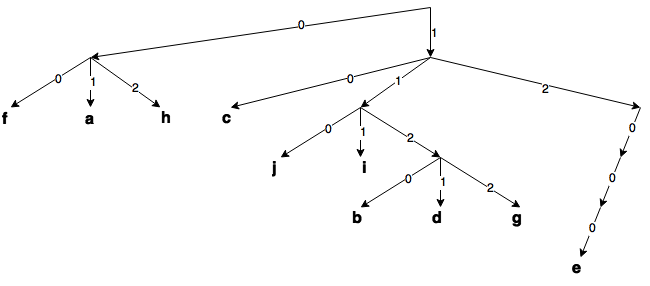
\includegraphics[width=0.6\textwidth]{img/shannon.png}
						\caption{Shannon-kód példa kódfája}
						\label{fig:shannon}
					\end{figure}
					
				\item[Huffman-kód] \hfill \\
					A Huffman-kód is optimális kód ($r$ elemszámú ábécével és $p_i$ gyakoriságokkal), melyet a következő módon állítunk elő. 
					\begin{enumerate}
						\item Rendezzük a betűket relatív gyakoriságaik alapján csökkenő sorrendbe.
						\item Annak érdekében, hogy csak egy csonka csúcs keletkezzen 
						\[m \equiv n \mod{r-1}\] 
						kongruenciának teljesülnie kell, ahol $m$ az egyetlen csonka csúcs kifoka. Ami ekvivalens azzal, hogy $m = 2 + ((n-2) \mod{r-1})$. Tehát osszuk el $n-2$-t $r-1$-gyel, és így $m$ a maradék+2 lesz.
						\item Az első lépésben a sorozat $m$ utolsó betűjét összevonjuk (új jelölést/betűt adunk neki), és ennek a relatív gyakorisága a tagok relatív gyakoriságának összege lesz. Rendezzük a sorozatot. Ezen lépés után már a betűk száma kongruens $r-1$-gyel, így a következő redukciós lépésekben mindig teljes csúcsokat tudunk készíteni.
						\item \label{itm:huffman_red} Az utolsó $r$ betűt vonjunk össze, helyettesítsük egy új betűvel és relatív gyakoriság legyen a relatív gyakoriságok összege.
						\item A \ref{itm:huffman_red}-beli redukciós lépést addig ismételjük míg $r$ db betű nem marad. Ekkor rendre minden betűhöz a kódábécé egy-egy betűjét rendeljük.
						\item \label{itm:huffman_split} Ha redukált elemmel találkozunk szétbontjuk, majd az ő elemeihez is a kódábécé betűit rendeljük, de konkatenáljuk az előzővel.
						\item A \ref{itm:huffman_split}-beli lépést addig ismételjük míg marad redukált elem.
					\end{enumerate}
					
					Példa:
					
					A Shannon-kódnál látott forrást kódoljuk be ugyanúgy $\{0,1,2\}$ kódábécével.
					
					\begin{tabular}{|c|c|c|c|c|c|c|c|c|c|}
						\hline a & b & c & d & e & f & g & h & i & j \\ 
						\hline 0,17 & 0,02 & 0,13 & 0,02 & 0,01 & 0,31 & 0,02 & 0,17 & 0,06 & 0,09 \\ 
						\hline 
					\end{tabular} 
					
					Rendezzük relatív gyakoriság szerint:
					
					\begin{tabular}{|c|c|c|c|c|c|c|c|c|c|}
						\hline f & a & h & c & j & i & b & d & g & e \\ 
						\hline 0,31 & 0,17 & 0,17 & 0,13 & 0,09 & 0,06 & 0,02 & 0,02 & 0,02 & 0,01 \\ 
						\hline 
					\end{tabular} 
					
					Osszuk el $n-2$-t $r-1$-gyel: $10-2 = 4*(3-1)+0$. Így $m$ a maradék+2, azaz $m=2$.
					Az utolsó $m$ betűt összevonjuk, és rendezzük a sorozatot:
					
					\begin{tabular}{|c|c|c|c|c|c|c|c|c|}
						\hline f & a & h & c & j & i & (g,e) & b & d  \\ 
						\hline 0,31 & 0,17 & 0,17 & 0,13 & 0,09 & 0,06 & 0,03 & 0,02 & 0,02 \\ 
						\hline 
					\end{tabular}
					
					Innentől kezdve minden redukciós lépésben az utolsó $r$ db azaz 3 betűt vonjuk össze:
					
					\begin{tabular}{|c|c|c|c|c|c|c|}
						\hline f & a & h & c & j & ((g,e), b, d) & i  \\ 
						\hline 0,31 & 0,17 & 0,17 & 0,13 & 0,09 & 0,07 & 0,06  \\ 
						\hline 
					\end{tabular}
					
					Ezt addig ismételjük, míg $r$ darab betű marad:
					
					\begin{tabular}{|c|c|c|}
						\hline (a,h,c) & f & (j,((g,e),b,d),i) \\ 
						\hline 0,47 & 0,31 & 0,22 \\ 
						\hline 
					\end{tabular} 
					
					A szétbontás alapján a \ref{fig:huffmann_split}. ábrán látható fát tudjuk összeállítani.
					
					\begin{figure}[H] 
						\centering
						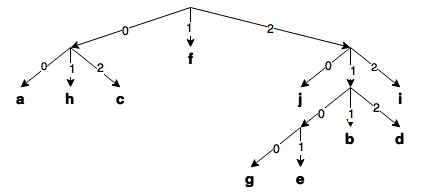
\includegraphics[width=0.6\textwidth]{img/huffmann_split.png}
						\caption{Huffman-kód példa kódfája}
						\label{fig:huffmann_split}
					\end{figure}
					
					Ezek alapján a kódtábla:
					
					\begin{tabular}{|c|c|c|}
						\hline betű & gyakoriság & kód \\
						\hline f & 0,31 & 1 \\ 
						\hline a & 0,17 & 00\\ 
						\hline h & 0,17 & 01\\ 
						\hline c & 0,13 & 02\\ 
						\hline j & 0,09 & 20\\ 
						\hline i & 0,06 & 22\\ 
						\hline b & 0,02 & 211\\ 
						\hline d & 0,02 & 212\\ 
						\hline g & 0,02 & 2100\\ 
						\hline e & 0,01 & 2101\\ 
						\hline 
					\end{tabular} 
			\end{description}
		\subsection{Hibajavító kódok, kódtávolság}
			\begin{description}
				\item[Hibakorlátozó kódolás] \hfill \\
					A hibakorlátozó kódokat két csoportba sorolhatjuk: hibajelző és  hibajavító kódok. Mindkét esetben az üzenetekhez kódszavakat rendelünk, amik alapján az átvitel során keletkező hibákat kezelni tudjuk. Ha az üzenet könnyen ismételhető hibajelző, ha nehezen ismételhető hibajavító kódot alkalmazunk. A hibakorlátozó kódoknál mindig azonos hosszúságú kódszavakat használunk. 
				\item[Kódok távolsága, súlya] \hfill \\
					A kódábécé $u$ és $v$ szavának Hamming-távolsága $d(u,v)$ az azonos pozícióban levő, eltérő jegyek száma.  A Hamming-távolság rendelkezik a távolság szokásos tulajdonságaival, vagyis $\forall u,v,z$:
					\begin{itemize}
						\item $d(u,v) \geq 0$
						\item $d(u,v) = 0 \ \Longleftrightarrow \ u = v$
						\item $d(u,v) = d(v,u)$ - szimmetria 
						\item $d(u,z) \leq d(u,v)+d(v,z)$ - háromszög egyenlőtlenség
					\end{itemize}
					A kód távolsága $d(C) = \min\limits_{u\neq v}d(u,v) \qquad (u,v \in C)$
					
					Amennyiben az $A$ kódábécé Abel-csoport a $0$ nullelemmel. Ekkor egy $u$ szó Hamming-súlya ($w(u)$) a szóban szereplő nem nulla elemek száma. Ekkor a kód súlya $w(C)  = \min\limits_{u\neq 0}w(u)$
				\item[Hibajavító kód] \hfill \\
					Amikor egy olyan szót kapunk, ami nem kódszó, a hozzá legkisebb Hamming-távolságú kódszóra javítjuk.
					
					A $K$ kód $t$-hibajavító, ha egy legfeljebb $t$ helyen megváltozott kódot helyesen javít. A $K$ kód pontosan $t$-hibajavító, ha $t$-hibajavító, de nem $t+1$-hibajavító.
					
					\textit{Megjegyzés: d minimális távolságú kód esetén d/2-nél kevesebb hibát biztosan egyértelműen tudunk javítani.}
				\item[Hamming-korlát] \hfill \\
					Egy $q$ elemű ábécé $n$ hosszú szavaiból álló $C$ kód $t$-hibajavító. Ekkor bármely két kódszóra a tőlünk legfeljebb $t$ távolságra lévő szavak halmazai diszjunktak.
					
					Mivel egy kódszótól $j$ távolságra pontosan $\binom{n}{j}(q-1)^j$ szó van, így a Hamming-korlát a kódszavak számára adott $t$-nél:
					\[\#(C) \cdot \sum\limits_{j=0}^{t}\binom{n}{j}(q-1)^j \leq q^n \]
					
					Amennyiben egyenlőség áll fent tökéletes kódról beszélünk.
			\end{description}
		\subsection{Lineáris kódok}
			\begin{description}
				\item[Definíció] \hfill \\
					$A$ véges test és $A^n$ lineáris tér. Minden $ K \leq A^n$ alteret lineáris kódnak nevezzük. Ha az altér $k$ dimenziós, a kód távolsága $d$ és $\#(A) = q$, akkor az ilyen kódot $[n,k,d]_q$ kódnak nevezzük.  	
					
					Egy lineáris kódnál feltesszük, hogy kódolandó üzenetek $K^k$ elemei, azaz a kódábécé elemeiből képzett $k$-asok.
				\item[Generátormátrix] \hfill \\
					$K$ véges test feletti $[n,k,d]_q$ lineáris kódolást válasszuk egy (kölcsönösen egyértelmű) lineáris leképezésnek:
					\[ G:K^k \rightarrow K^n \] 
					Ezt egy mátrixszal, az úgy nevezett generátormátrixszal jellemezhetjük.
				\item[Polinomkódok] \hfill \\
					Egy lineáris kód esetén az üzeneteket megfeleltethetjük $\mathbb{F}_q$ ($q$ elemű véges test) feletti $k$-nál alacsonyabb fokú polinomoknak. 
					\[(a_0,a_1,\cdots,a_{k-1}) \rightarrow a_0+a_1x+\cdots+a_{k-1}x^{k-1} \]
					
					Legyen $g(x)$ rögzített $m$-edfokú polinom. A $p(x)$ polinomot (üzenet) $g(x)$-szel szorozva lineáris kódolást kapunk (mivel a $p \rightarrow pg$ kölcsönösen egyértelmű). Ekkor a kódszavak hossza $n=k+m$. Az ilyen típusú lineáris kódolást polinomkódolásnak nevezzük.
					
					\textit{Megjegyzés: Feltehetjük, hogy $g(x)$ főpolinom (együtthatója egység), illetve a konstans tag nem nulla (ha nulla lenne, a szorzatban kiesne a konstans tag, így a kódban a nulla indexű betű soha nem hordozna információt)}
				\item[CRC - Cyclic Redundancy Check] \hfill \\
					Ha egy polinomkódban $g(x) | x^n-1$, akkor ciklikus kódról beszélünk. Ekkor, ha $a_0a_1\cdots a_{n-1}$ kódszó, akkor $a_{n-1}a_0\cdots a_{n-2}$ is az, mivel:
					\[ a_{n-1}+a_0x+\cdots+a_{n-2}x^{n-1} \ = \ x\cdot(a_0+a_1x+\cdots a_{n-1}x^{n-1})-a_{n-1}(x^n-1) \]
					osztható $g(x)$-szel.
					
					A CRC az $\mathbb{F}_2$ feletti ciklikus kódokat foglalja magába. Csak hibajelzésre alkalmas, a kódolás a következő: Vegyük $p(x)x^m = (0,0,\cdots,0,a_m,a_{m+1},\cdots,a_{n-1})$. Ezt osszuk el $g(x)$-el maradékosan. $p(x)x^m = q(x)g(x)+r(x)$. Ekkor a kódszó legyen: $p(x)x^m-r(x) = q(x)g(x)$, amely osztható $g(x)$-szel és magas fokszámokon az eredeti üzenet betűi helyezkednek el. A vett szó ellenőrzése egyszerű: Megnézzük, hogy osztható-e $g(x)$-szel, ha nem, hiba történt.
			\end{description}
\end{document}